
\chapter{Introduzione}


La crittografia è un metodo per un utente di condividere in maniera sicura i propri dati su un mezzo di comunicazione o un sito insicuri.\\
Prima della crittografia a chiave pubblica, un metodo ampiamente utilizzato tra due utenti per comunicare informazioni confidenziale era quello di stabilire a priori un segreto comune e ben protetto che permettesse di decodificare le informazioni.\\
Nonostante questo metodo possa esser accettabile per piccoli gruppi diventa obsoleto ed inutilizzabile in una infrastuttura molto grande come quella di Internet che conta miliardi di utenti.\\

Quasi 40 anni fa, Diffie ed Hellman pubblicarono una rivoluzionaria idea racchiusa nel concetto di \emph{crittografia a chiave pubblica}:\\
{ \itshape due gruppi possono comunicare in maniera sicura senza dover accordarsi su un segreto comune.}

\vspace{0.4cm}

Al giorno d'oggi la crittografia a chiave pubblica è uno strumento fondamentale e il suo utilizzo è centrale per la communicazione sicura via web, alla cifratura di dischi e per la possibilità di garantire l'autenticità di persone.\\
Comunque vi sono delle particolarità:
\begin{itemize}
	\item Crittare è un metodo per inviare un messggio ad \textbf{una singola} entità che detiene una chiave segreta
	\item L'accesso ai dati cifrati è totale o nulla : una persona può decifrare e leggere completamente il messaggio \textbf{o} non può nemmeno decifrarlo.
\end{itemize}

La combinazione di questi due punti ci porta a dover rispondere ad un problema molto particolare:

\begin{center}
{\itshape È possibile costruire un sistema crittografico dove sia possibile crittare \textbf{una} volta sola il messaggio per poi distribuirla a più persone creando la possibilità di filtrare il contenuto in base alla persona che cerca di decifrarla?}
\end{center}

Se dovessimo utilizzare la normale assunzione DH con chiavi pubbliche, avremo ad esempio un sistema di questo tipo:

\begin{center}
\begin{minipage}[c]{0.9\textwidth}
		\centering
		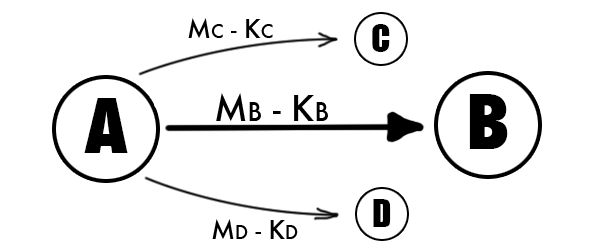
\includegraphics[keepaspectratio,width=\textwidth]{keying.png}\\
		{\small\scshape Un utente, tante chiavi per ogni utente}
\end{minipage}
\end{center}

Dove siamo costretti ad avere molte chiavi diverse per permettere la comunicazione verso ogni destinatario. Il messaggio viene crittato tante volte quanti sono i destinatari.\\[0.3cm]

Per questo motivo, Sahai and Waters \cite{sahai} fanno i primi passi per risolvere il problema intriducendo il concetto di ABE : Attribute Based Encryption.\\
Questo schema prevede la definizione di un insieme di attributi che funzioneranno da etichettatura per ogni messaggio crittato.\\
La chiave di decifratura (privata) verrà calcolata per ogni utente in base agli attributi che quell'utente ha diritto a visionare: viene così creata una vera e propria policy d'accesso differenziata per ogni utente.\\
A questo punto, l'utente è in grado di crittare il messaggio \emph{attaccandogli} gli attributi che preferisce. Questi attributi definiranno quali utenti potranno decifrare il messaggio: le chiavi che rispettano la policy, utilizzando gli attributi del messaggio, hanno diritto e possono decrittarlo.\\[0.2cm]

\begin{center}
\begin{minipage}[c]{0.9\textwidth}
		\centering
		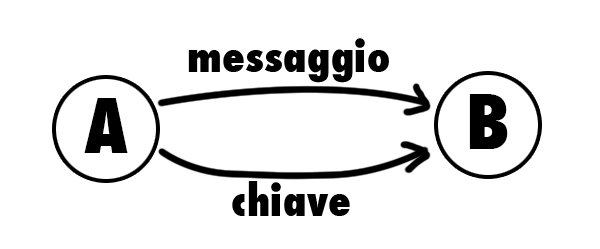
\includegraphics[keepaspectratio,width=\textwidth]{pairing.png}\\
		{\small\scshape Un utente, un messaggio con le etichette, tanti utenti caratterizzati}
\end{minipage}
\end{center}

\vspace{0.3cm}

La nascità dei servizi \emph{cloud} aumenta la necessità di risolvere il problema difficilmente risolvibile dalla crittografia a chiave publica.\\
Un esempio concreto: consideriamo un servizio di memorizzazione in cloud che immagazzina immagini. Le forze dell'ordine potrebbero aver bisogno di cercare sul cloud un immagine contenente un particolare volto.\\
Il cloud necessita una chiave segreta per l'occasione che sia in grado di decifrare le immagini che contengono la faccia cercata ma che non visualizzi il resto delle immagini.\\[0.2cm]

Data la necessità di creare sistemi di crittografia che rispondessero a queste esigenze odierne, vi sono stati molti tentativi di una costruzione matematica che rispondesse alle esigenze. Quello studiato in questa tesi è \cite{kpabe}.\\
Lo strumento principale tra tutte queste costruzioni è un pairing $e$ tra gruppi ciclici.\\
Questo pairing deve avere proprietà particolari (vedi \ref{pairinge}).\\
Esistono pairing molto complessi \cite{maas} \cite{benoit} tra cui il pairing di Tate e il pairing di Weil.\\[0.2cm]
Nello studio di questa tesi, sono stati evidenziati due diverse metodologie di crittografia:
\begin{itemize}
	\item \textbf{Identity Based Encryption} : Un garante genera per ogni utente delle chiavi private che vengono concesse unicamente se l'utente viene autenticato. A questo punto ogni utente autenticato avrà una propria chiave privata e pubblica dove questa seconda sarà possibile calcolarla on-the-fly senza dover esser salvata. Con queste chiavi è possibile comunicare firmando e crittando i messaggi.\\
	Questo metodo, ideato temporalmente prima degli altri, è molto problematico e risente di difficoltà pratiche che lo rendono inutilizzabile per un applicazione reale.
	\item \textbf{Attribute Based Encryption} : Il sistema conosce a priori \emph{quanti} attributi gestirà. Da questi vengono create delle chiavi pubbliche che sono l'insieme di \emph{sottochiavi} per ogni singolo attributo. In questo modo ogni messaggio che viene cifrato, subisce una trasformazione \emph{neutra} rispetto agli attributi quando questi saranno fondamentali per decretare o meno l'autorizzazione a decifrare.
\end{itemize}

Nella prima, l'identità di una persona definisce la chiave rendendo il modello molto simile alla crittografia a chiave pubblica con la capacità di risolvere il problema principale in maniera teorica seppur con qualche problema pratico.\\
Nel secondo, gli attributi non definiscono chiavi ma bensì delle policy d'accesso. In questo modo chiavi e attributi si separano concettualmente risolvendo il problema.\\
Altre differenze dettagliate si possono trovare a \ref{ibeabe}\\[0.2cm]

Questo schema crittografico non è ancora pienamente conosciuto ed è per questo difficile definire e garantire un livello di sicurezza adatto per poter esser utilizzato nella quotidianità, come spiegato a \ref{secur}.\\[0.2cm]

In questa tesi verrà studiato lo schema ABE descritto in \cite{kpabe}.








% \begin{defi}
% Coefficente di Lagrange
% \[ \Delta_{i,s}(x) = \prod_{j\in S , j \neq i} \dfrac{x-j}{i-j} \]
% \end{defi}
